\chapter{Análise de desempenho}

A implementação do protótipo foi testada em diversas conexões com a \textit{internet}, tanto institucionais, como a rede da Universidade de São Paulo, quanto residenciais e móveis. Como o \textit{UPnP} não é universalmente compatível com todos os roteadores, a maior parte dos testes que utilizaram \textit{UPnP} foi realizada em conexões residenciais de uma empresa que tem roteadores compatíveis com o protocolo. Como a rede do \textit{Tor} não é restrita no Brasil, em nenhuma das conexões testadas houve problemas de acesso aos serviços ocultos de outros usuários. Os resultados dos experimentos realizados para avaliar o desempenho da proposta apresentam algumas considerações sobre as limitações deste protótipo.

\section{Tempo de inicialização do \textit{Tor}}

O tempo de inicialização do \textit{Tor} é uma inconveniência para a mobilidade deste protocolo. Enquanto esse programa termina de se inicializar em menos de 10 segundos na maioria dos casos, os serviços ocultos que são hospedados por ele demoram mais para serem adicionados à Tabela de \textit{Hash} Distribuída do protocolo. Quando o \textit{Tor} tenta acessar um serviço oculto que ainda não terminou de ser inicializado, ele demora muito para desistir da tentativa de conexão, gerando uma má experiência ao usuário. Por causa disso, é importante que o usuário espere pelo menos um minuto depois da inicialização completa do servidor para tentar se comunicar com outros usuários.

Uma vez que a conectividade pelo \textit{Tor} é essencial ao protocolo, mesmo em casos em que os usuários estão se comunicando de forma \textit{P2P}, é importante que o usuário tenha uma conexão estável com a rede do \textit{Tor}. Isso torna este protótipo inconveniente e imprático para utilização em movimento, como em um \textit{smartphone}, por exemplo.

\section{Limitações do \textit{UPnP}}

O \textit{UPnP} é um protocolo que não é universalmente compatível com todos os roteadores. Em alguns casos, o \textit{UPnP} não é habilitado por padrão, e em outros casos, o roteador não é compatível com o protocolo. Enquanto seria possível implementar instruções para o usuário manualmente abrir portas em seu roteador, isto é uma inconveniência e não foi implementado neste protótipo. Quando a conexão \textit{P2P} não é possível, como por exemplo nesse caso, o programa simplesmente continua se comunicando com outros usuários através do \textit{Tor}.

Inicialmente, o programa utilizaria a biblioteca \textit{miniupnpc} para abrir portas automaticamente, porém, ao longo dos testes, ela apresentou problemas relacionados com o \textit{timeout} de tentativas de conexão com o roteador. Esta biblioteca, ao tentar descobrir dispositivos compatíveis com \textit{UPnP} na rede, ficava indefinidamente esperando por uma resposta, tornando o processo de descoberta de dispositivos \textit{UPnP} extremamente demorado. Por causa disso, o arquivo \textit{upnp.py} apresenta uma implementação própria que utiliza o executável \textit{upnpc}, que não sofre com este problema específico. Por outro lado, o executável \textit{upnpc} também apresentava problemas de inconsistência na resposta de pedidos. Pedidos para a abertura de portas específicas entravam na tabela de roteamento, mas não estavam ativos. Além disso, muitos comandos terminavam com códigos de erro, mesmo tendo sido bem-sucedidos. Assim, a implementação teve que manualmente testar se os comandos executados eram bem-sucedidos, limpando todos os roteamentos pedidos quando encontrava um erro.

\section{Velocidade de conexões e latência}

Como a implementação prática do protocolo apenas permite o envio de mensagens de texto, que ocupam muito pouco espaço em disco, a velocidade da conexão entre dois usuários é em grande parte irrelevante. O parâmetro mais importante que foi analisado foi a latência de envio de mensagens entre os dispositivos. Para cada ação entre dispositivos foram coletadas 6 medidas de latência, e a média dessas medidas foi utilizada como a latência da conexão. As Tabelas \ref{tab:latencia_handshake} e \ref{tab:latencia_mensagens} apresentam os resultados dessas medições. Como mencionado anteriormente, como o \textit{Tor} demora para tornar os serviços ocultos acessíveis externamente, os programas foram iniciados e os testes só foram conduzidos depois de 1 minuto.

\begin{table}[H]
\centering
\begin{tabular}{|c|c|c|}
\hline
\textbf{Ação} & \textbf{Tempo Médio} & \textbf{Desvio Padrão} \\ \hline
Pedido da chave pública do destinatário & 5.94s & 0.83s \\ \hline
\textit{Handshake} inicial entre dois clientes & 13.82s & 1.77s \\ \hline
\end{tabular}
\caption{Medições de latência para pedido da chave pública e \textit{handshake}}
\label{tab:latencia_handshake}
\end{table}

\begin{table}[H]
\centering
\begin{tabular}{|c|c|c|}
\hline
\textbf{Ação} & \textbf{Tempo Médio} & \textbf{Desvio Padrão} \\ \hline
Envio de mensagens (\textit{Tor}) & 1740ms & 220ms \\ \hline
Envio de mensagens (\textit{UPnP}) & 5.83ms & 0.75ms \\ \hline
Envio de mensagens (Rede local) & 2.33ms & 0.52ms \\ \hline
Envio de mensagens (\textit{localhost}) & 8ms & 1.41ms \\ \hline
\end{tabular}
\caption{Medições de latência para envio de mensagens}
\label{tab:latencia_mensagens}
\end{table}

As máquinas utilizadas para estes testes contém as seguintes especificações técnicas:

Máquina 1:

\begin{tcolorbox}[colback=gray!10, colframe=gray, sharp corners=south]
\begin{itemize}
    \setlength\itemsep{0em}
    \setlength\leftmargini{2em}
    \item Servidor montado para hospedar websites e armazenar aquivos em uma conexão residencial
    \item Processador: AMD Ryzen 5 1600 AF
    \item Memória: 16GB DDR4 2666MHz ECC
    \item Armazenamento: SSD NVMe 256GB
    \item Sistema Operacional: Debian Linux 12 Bookworm
    \item Conexão com a \textit{Internet}: Conexão residencial de fibra ótica com 600MBits/s (Download) e 300MBits/s (Upload)
\end{itemize}
\end{tcolorbox}

Máquina 2:

\begin{tcolorbox}[colback=gray!10, colframe=gray, sharp corners=south]
\begin{itemize}
    \setlength\itemsep{0em}
    \setlength\leftmargini{2em}
    \item Laptop para uso pessoal (Thinkpad L14 Gen 3)
    \item Processador: AMD Ryzen 5 5500U
    \item Memória: 16GB DDR4 3200MHz
    \item Armazenamento: SSD NVMe 256GB
    \item Sistema Operacional: Manjaro Linux 24.2.0 (Gnome)
    \item Conexão com a internet: Mesma que a Maquina 1 (Testes de rede local) através de cabo de rede, e conexão com a rede Wi-Fi Eduroam da USP (Testes de rede externa)
\end{itemize}
\end{tcolorbox}

O envio de mensagens através do \textit{Tor} passa as mensagens por 6 computadores da rede do \textit{Tor} antes que a mensagem seja entregue, tornando este método de conexão o mais limitado em latência. Uma consideração interessante é que, por causa do \textit{handshake} inicial do \textit{Tor}, a primeira conexão é muito mais demorada do que as demais. Uma vez que ambos os servidores já se comunicaram, seu caminho fica armazenado, tornando conexões posteriores muito mais rápidas. Por causa disso, o pedido da chave pública (que é o primeiro passo no envio da primeira mensagem entre dois usuários) e o \textit{handshake} (que é o primeiro pedido no sentido contrário do que a mensagem será enviada) são muito mais lentos do que o envio de mensagens subsequentes.

De forma muito interessante, o envio de mensagens através de \textit{UPnP} e rede local é mais rápido do que o envio de mensagens através de \textit{localhost}. Isso se deve ao fato de que mensagens enviadas pelo \textit{localhost} utilizam a biblioteca de \textit{Python Requests}, que é complexa e mais lenta, enquanto pedidos enviados pela rede local e \textit{UPnP} são enviados diretamente para o \textit{socket}, sem intermediários. O envio de mensagens através de \textit{UPnP} é mais lento do que o envio de mensagens pela rede local por causa da latência da comunicação através da \textit{internet}. De qualquer maneira, nos três casos, o envio das mensagens é extremamente rápido, apenas demorando alguns milissegundos.

Os resultados desses testes foram realizados em situações bem ideais de rede, com conexões cabeadas e provedores de \textit{internet} de alta qualidade. Condições adversas de rede definitivamente alterarão esses resultados.

\begin{figure}[H]
\centering
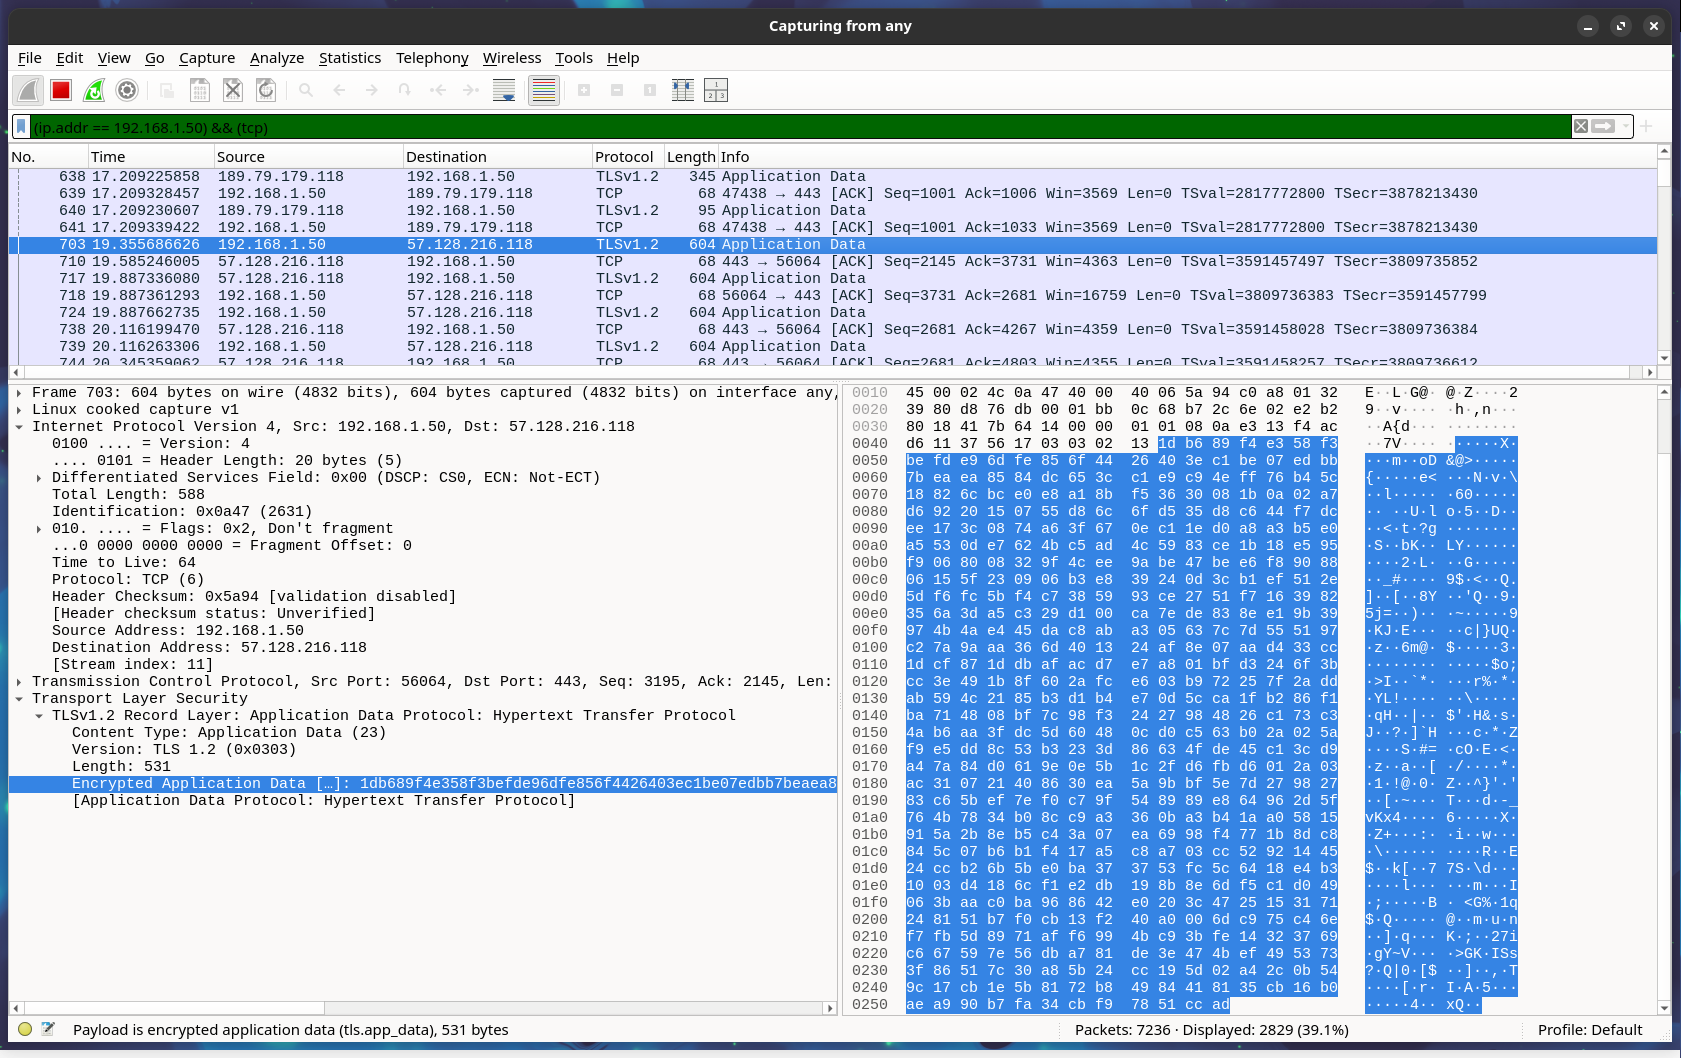
\includegraphics[width=0.95\textwidth]{packet-tor.png}
\caption{Captura de tela do Wireshark mostrando um pacote criptografado pelo \textit{Tor}. Note que o conteúdo do pacote é criptografado, e aparece portanto como uma série de caracteres aleatórios. A barra mais a direita, sublinhada em azul, contém o conteúdo do pacote em hexadecimal e sendo interpretado como texto.}
\label{fig:packet-tor}
\end{figure}

\begin{figure}[H]
\centering
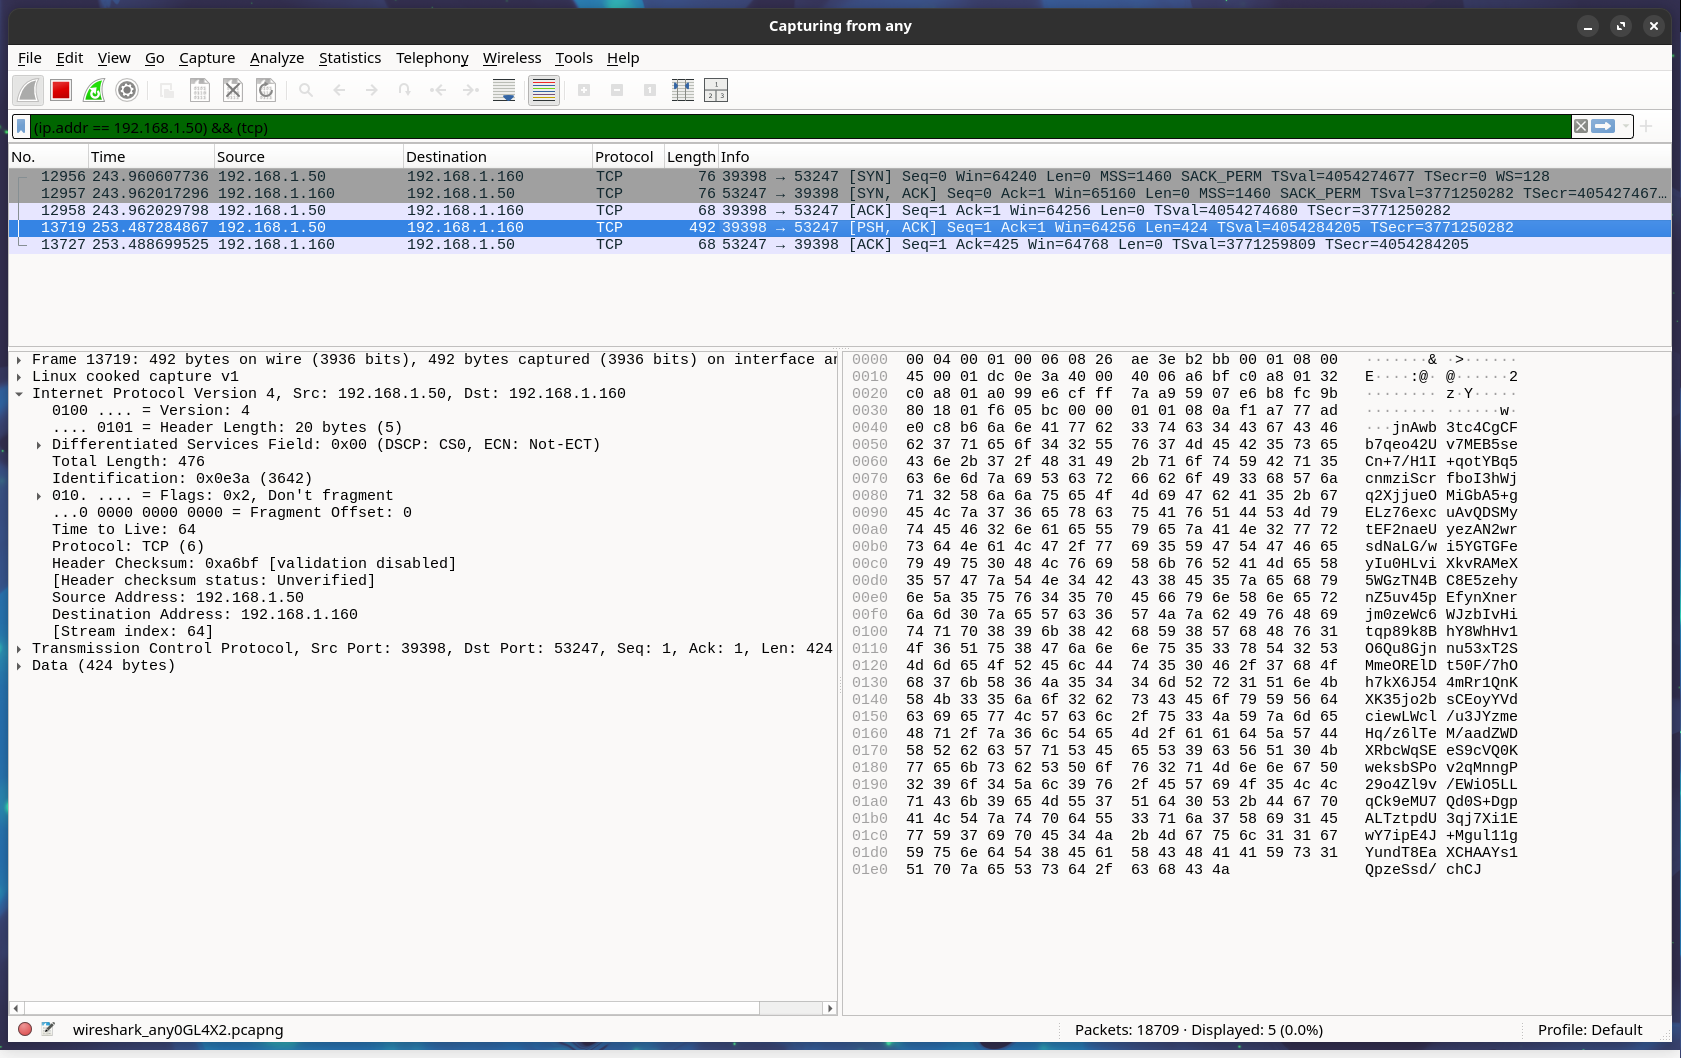
\includegraphics[width=0.95\textwidth]{packet-local.png}
\caption{Captura de tela do Wireshark mostrando um pacote criptografado pelo protótipo em uma conexão entre amigos em uma rede local. O conteúdo do pacote é texto criptografado, e depois codificado em base64. Por isso, o conteúdo do pacote é ilegível a uma pessoa não autorizada.}
\label{fig:packet-local}
\end{figure}

\begin{figure}[H]
\centering
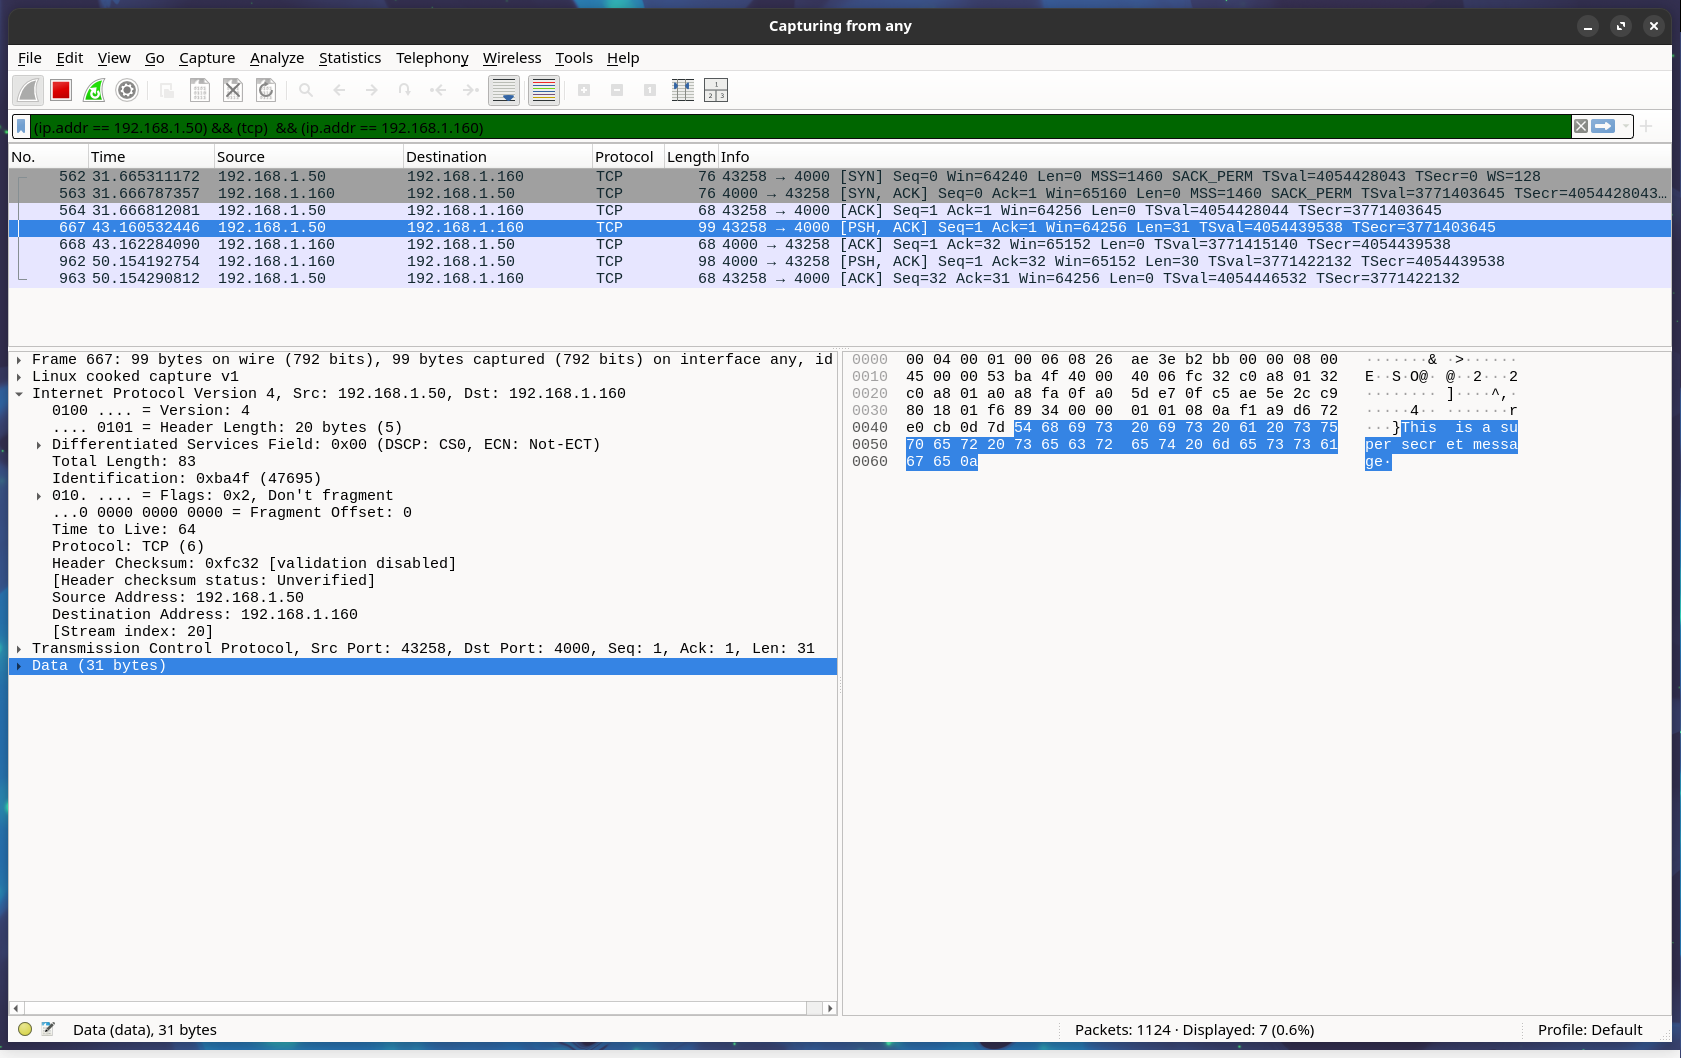
\includegraphics[width=1\textwidth]{packet-plaintext.png}
\caption{Captura de tela do Wireshark mostrando um pacote de dados não criptografado como exemplo. Neste caso, é possível ver o conteúdo do pacote em texto, na direita da tela.}
\label{fig:packet-plaintext}
\end{figure}

As Imagens \ref{fig:packet-tor}, \ref{fig:packet-local}, e \ref{fig:packet-plaintext} mostram capturas de tela do programa Wireshark, que é um programa de análise de pacotes de rede. Ele permite analisar tráfego que é acessível pelas interfaces de rede da máquina em que ele roda. Neste exemplo, ele é utilizado para demonstrar como o tráfego gerado pelo protótipo não pode ser decodificado por atores mal intencionados. A Imagem \ref{fig:packet-tor} mostra um pacote criptografado pelo \textit{Tor}, que é ilegível a uma pessoa não autorizada. A Imagem \ref{fig:packet-local} mostra um pacote criptografado pelo protótipo em uma conexão entre amigos em uma rede local, que é codificado em base64 e também ilegível a uma pessoa não autorizada. A Imagem \ref{fig:packet-plaintext} mostra um pacote qualquer de dados não criptografados, que é legível a qualquer pessoa que tenha acesso ao pacote.